% Copyright (c) 2019 Bochen Tan
% Public domain.
%本模板的宗旨是尽量绿色,不需要附加安装任何东西。
%按照教务部下发的WORD说明文档格式,下简称“说明”
%没有封面和评阅表,这两部分请直接在Cover&ReviewTable.doc中写再输出pdf拼到一起
%doc小改动:封面校徽和文字替换为了高清版本,“题目:”和中文题目对齐,中英文题目分在了表的两行
%doc小改动:插入了两个白页,使得连续打印的时候封面和表格都在奇数页
%正文部分改动:在每一页下方中央加了页码,因为说明中页眉不分奇偶页,所以页码就都在中央吧
%不含自动的参考文献,因为说明中参考文献格式不典型,请手动输入或自行写程序
%在Windows或Linux下渲染出字体更接近说明,Mac OS上字体不太一样
%有警告\headheight is too small,fancyhdr的上距离有点小,似乎问题不大

\documentclass[UTF8,openany,AutoFakeBold,AutoFakeSlant,cs4size]{ctexbook}
%openany 使一章可以从偶数页开始,因为说明中每一章并没有只能从奇数页开始,虽然这是常理
%AutoFakeBold 和 AutoFakeSlant 因为 CJK 里没有真正的加粗和倾斜,如果额外字体则效果更好
%cs4size 因为要求主题是小四号字

\usepackage[a4paper,left=3.18cm,right=3.18cm,top=2.54cm,bottom=2.54cm]{geometry}
%office中正常页边距



\usepackage{amsmath}
\usepackage{amsthm}
\usepackage{bm}
\usepackage{amsfonts}
\usepackage{enumerate}
\usepackage{fancyhdr}
\usepackage{color}
\usepackage{proof}



\usepackage{cite}
\newcommand{\upcite}[1]{\textsuperscript{\cite{#1}}} %引用在右上角

\usepackage{hyperref}
\usepackage{gbt7714}

\usepackage{multirow,booktabs,makecell}
\usepackage{graphicx}
\usepackage[font=small,labelsep=space]{caption} %五号,宋体/Time new roman
\renewcommand{\thetable}{\arabic{table}} %表格和图片编号不分章节,直接1,2,3 ...
\renewcommand{\thefigure}{\arabic{figure}}
\renewcommand{\theequation}{\arabic{chapter}.\arabic{equation}} %公式标签 章.公式(均为阿拉伯数字)



\usepackage{tocloft} %自定义目录,说明中没有明确规定,和WORD自动生成目录格式一致

%“全文目录”四个字的格式
\renewcommand\cftbeforetoctitleskip{0pt}
\renewcommand\cftaftertoctitleskip{0pt}
\renewcommand\cfttoctitlefont{\bfseries\heiti\zihao{2}}

\renewcommand\cftchapfont{\heiti\normalsize} %黑体小四
\renewcommand\cftchapdotsep{\cftdotsep} %有点连到页码,点间距不确定,待改
\renewcommand\cftchappagefont{\songti\normalsize} %宋体小四页码
\renewcommand\cftbeforechapskip{0pt}

%1. 第一级 五号宋体,缩进两个字符,页码一致
\renewcommand\cftsecfont{\songti\small}
\renewcommand\cftsecpagefont{\songti\small}
\renewcommand\cftsecaftersnum{.} %一级目录号后加点
\renewcommand\cftsecindent{2em}
\renewcommand\cftbeforesecskip{0pt}

%1.1 第二级 五号宋体,缩进四个字符,页码一致
\renewcommand\cftsubsecfont{\songti\small}
\renewcommand\cftsubsecpagefont{\songti\small}
\renewcommand\cftsubsecindent{4em}
\renewcommand\cftbeforesubsecskip{0pt}

%1.1.1 第二级 五号宋体,缩进四个字符,页码一致
\renewcommand\cftsubsubsecfont{\songti\small}
\renewcommand\cftsubsubsecpagefont{\songti\small}
\renewcommand\cftsubsubsecindent{4em}
\renewcommand\cftbeforesubsubsecskip{0pt}



\usepackage{titlesec}%自定义章节标题
\CTEXsetup[format={\bfseries\center\heiti\zihao{2}},beforeskip=0pt]{chapter}
%第一章  绪论(二号、黑体) beforeskip为上方垂直距离看起来还比说明偏大,待改

\setcounter{tocdepth}{3}
\setcounter{secnumdepth}{3}
%使目录中有三级标题,即subsubsection

\renewcommand\thesection{\arabic{section}} % 使得不显示章名,只显示节名
\titleformat{\section}
{\raggedright\zihao{3}\bfseries\songti}
{\thesection.\quad}
{0pt}
{}%1. 第一级(三号、宋体/Time new roman、加粗)

\titleformat{\subsection}
{\raggedright\bfseries\zihao{4}\songti}
{\thesubsection\quad}
{0pt}
{}%1.1 第二级(四号,宋体/Time new roman,加粗)

\titleformat{\subsubsection}
{\raggedright\bfseries\zihao{-4}\songti}
{\thesubsubsection\quad}
{0pt}
{}%1.1.1 第三级(小四,宋体/Time new roman,加粗)




% 封面依赖的宏包
\usepackage{xcoffins} % 用于设计封面格式
\usepackage{xcolor}
\usepackage{xeCJK} % 用于引入楷体
\usepackage{soul} % 用于设置下划线宽度
\setul{}{2pt}
\setmainfont{Times New Roman} % Times New Roman 作为默认英文字体
% 引入楷体,请改成自己系统里对应的名字
\setCJKfamilyfont{kaiti}[AutoFakeBold=1.5]{楷体}
\newcommand{\kaiti}{\CJKfamily{kaiti}}

% 评阅表依赖的宏包
\usepackage{float}
\usepackage{array}



\title{}
\author{}
\date{}
\begin{document}

% 封面中需要修改的内容直接在此处更改即可
\newcommand{\chineseTitle}{一种利用Redex实现重组糖的轻量级方法}
\newcommand{\englishTitle}{A Lightweight Resugaring Method using PLT Redex}
\newcommand{\name}{杨子毅}
\newcommand{\studentID}{1600011063}
\newcommand{\school}{信息科学技术学院}
\newcommand{\major}{软件工程}
\newcommand{\advisor}{胡振江}
% 插入封面
% 声明需要的Coffin
\NewCoffin \result
\NewCoffin \topBox
\NewCoffin \badge
\NewCoffin \pku
\NewCoffin \headingText
\NewCoffin \titleText
\NewCoffin \chineseTitleText
\NewCoffin \englishTitleText
\NewCoffin \nameText
\NewCoffin \studentIDText
\NewCoffin \schoolText
\NewCoffin \majorText
\NewCoffin \advisorText
\NewCoffin \dateText


% 各个Coffin的内容
\SetHorizontalCoffin \result {}
\SetHorizontalCoffin \topBox {\color{white} \rule{210mm}{41mm}}
\SetHorizontalCoffin \badge {
\includegraphics[width=20.6mm]{images/badge}}
\SetHorizontalCoffin \pku {
\includegraphics[width=60.5mm]{images/pku}}
\SetVerticalCoffin \headingText{160mm}{\center\heiti\fontsize{36}{36}\textcolor{black}{本科生毕业论文}}
\SetVerticalCoffin \titleText{22mm}{\bfseries\songti\zihao{3}{题目:}}
\fontsize{22}{22}\selectfont
\SetVerticalCoffin \chineseTitleText{130mm}{\bfseries\kaiti\underline{\makebox[142mm][l]{\chineseTitle}}}
\SetVerticalCoffin \englishTitleText{130mm}{\bfseries\kaiti\zihao{3}\underline{\makebox[122mm][l]{\englishTitle}}}
\fontsize{16}{16}\selectfont
\SetVerticalCoffin \nameText{104mm}{\center\songti\textcolor{black}{姓\qquad 名:\underline{\makebox[76mm][c]{\kaiti{\name}}}}}
\SetVerticalCoffin \studentIDText{104mm}{\center\songti\fontsize{16}{16}\textcolor{black}{学\qquad 号:\underline{\makebox[76mm][c]{\kaiti\zihao{3}{\studentID}}}}}
\SetVerticalCoffin \schoolText{104mm}{\center\songti\fontsize{16}{16}\textcolor{black}{院\qquad 系:\underline{\makebox[76mm][c]{\kaiti{\school}}}}}
\SetVerticalCoffin \majorText{104mm}{\center\songti\fontsize{16}{16}\textcolor{black}{本科专业:\underline{\makebox[76mm][c]{\kaiti{\major}}}}}
\SetVerticalCoffin \advisorText{104mm}{\center\songti\fontsize{16}{16}\textcolor{black}{指导老师:\underline{\makebox[76mm][c]{\kaiti{\advisor}}}}}
\fontsize{18}{18}\selectfont
\SetVerticalCoffin \dateText{104mm}{\center\kaiti\textcolor{black}{二〇二〇\quad 年\quad 五\quad 月}}


% 指定各个Coffin相对位置关系
\JoinCoffins \result \topBox
\JoinCoffins \result[\topBox-hc, \topBox-b] \badge[r, b](-27.9mm, -20.6mm)
\JoinCoffins \result[\topBox-hc, \topBox-b] \pku[l, b](-11.3mm, -20.6mm)
\JoinCoffins \result[\topBox-hc, \topBox-b] \headingText[hc, b](0mm, -63.8mm)
\JoinCoffins \result[\headingText-hc, \headingText-b] \titleText[l, t](-73.25mm, -20mm)
\JoinCoffins \result[\headingText-hc, \headingText-b] \chineseTitleText[l, t](-57.85mm, -18.85mm)
\JoinCoffins \result[\headingText-hc, \headingText-b] \englishTitleText[l, t](-49.85mm, -34mm)
\JoinCoffins \result[\headingText-hc, \headingText-b] \nameText[hc, t](0mm, -60mm)
\JoinCoffins \result[\nameText-hc, \nameText-b] \studentIDText[hc, t](0mm, 0mm)
\JoinCoffins \result[\studentIDText-hc, \studentIDText-b] \schoolText[hc, t](0mm, 0mm)
\JoinCoffins \result[\schoolText-hc, \schoolText-b] \majorText[hc, t](0mm, 0mm)
\JoinCoffins \result[\majorText-hc, \majorText-b] \advisorText[hc, t](0mm, 0mm)
\JoinCoffins \result[\advisorText-hc, \advisorText-b] \dateText[hc, t](0mm, -20mm)


% 输出封面
\thispagestyle{empty}
\newgeometry{left=0mm,bottom=0mm, top=0mm, right=0mm}
\noindent\TypesetCoffin \result
\restoregeometry
\clearpage


% 插入导师评阅表
\thispagestyle{empty}
\newgeometry{left=2cm, right=2cm, top=2.64cm, bottom=2.54cm}
\renewcommand\arraystretch{1.2}

\begin{center}
{\songti\zihao{3}{北京大学本科毕业论文导师评阅表}}
\end{center}

\begin{table}[H]
	\centering
    \begin{tabular}{|rrrrrr|}
    \hline
    \multicolumn{1}{|p{4em}|}{学生姓名} & \multicolumn{1}{p{3em}|}{} & \multicolumn{1}{p{5em}|}{学生学号} & \multicolumn{1}{p{6.5em}|}{} & \multicolumn{1}{p{6.565em}|}{论文成绩} &  \multicolumn{1}{r|}{}\\
    \hline
    \multicolumn{1}{|p{4em}|}{学院(系)} & \multicolumn{3}{r|}{} & \multicolumn{1}{p{6.565em}|}{学生所在专业} &  
    \multicolumn{1}{r|}{}\\
    \hline
    \multicolumn{1}{|r|}{\multirow{2}[2]{*}{导师姓名}} & \multicolumn{1}{r|}{\multirow{2}[2]{*}{}} & \multicolumn{1}{p{5em}|}{导师单位/} & \multicolumn{1}{r|}{\multirow{2}[2]{*}{}} & \multicolumn{1}{p{6.565em}|}{\multirow{2}[2]{*}{导师职称}} & \multirow{2}[2]{*}{} \\
    \multicolumn{1}{|r|}{} & \multicolumn{1}{r|}{} & \multicolumn{1}{p{5em}|}{所在研究所} & \multicolumn{1}{r|}{} & \multicolumn{1}{r|}{} &  \\
    \hline
    \multicolumn{2}{|p{9em}|}{\centering{论文题目}} & \multicolumn{4}{r|}{\multirow{2}[2]{*}{}} \\
    \multicolumn{2}{|p{9em}|}{\centering{(中、英文)}} & \multicolumn{4}{r|}{} \\
    \hline
    \multicolumn{6}{|p{35.88em}|}{\center{导师评语}} \\
    \multicolumn{6}{|p{35.88em}|}{\kaiti{(包含对论文的性质、难度、分量、综合训练等是否符合培养目标的目的等评价)}} \\
    \multicolumn{6}{|c|}{} \\
    \multicolumn{6}{|c|}{} \\
    \multicolumn{6}{|c|}{} \\
    \multicolumn{6}{|c|}{} \\
    \multicolumn{6}{|c|}{} \\
    \multicolumn{6}{|c|}{} \\
    \multicolumn{6}{|c|}{} \\
    \multicolumn{6}{|c|}{} \\
    \multicolumn{6}{|r|}{} \\
    \multicolumn{6}{|r|}{} \\
    \multicolumn{6}{|r|}{} \\
    \multicolumn{6}{|r|}{} \\
    \multicolumn{6}{|r|}{} \\
    \multicolumn{6}{|r|}{} \\
    \multicolumn{6}{|r|}{} \\
    \multicolumn{6}{|p{35.88em}|}{                                                                             \hfill 导师签名:\qquad\qquad\qquad\qquad\qquad\qquad\qquad\qquad } \\
    \multicolumn{6}{|r|}{} \\
    \multicolumn{6}{|p{35.88em}|}{\hfill 年 \qquad\quad 月 \qquad\quad 日 \qquad\qquad\qquad} \\
    \multicolumn{6}{|r|}{} \\
    \hline
    \end{tabular}
\end{table}

\renewcommand\arraystretch{1}
\restoregeometry
\clearpage

\zihao{-4}\songti\linespread{1.5}\selectfont
\linespread{1.5}\selectfont
\chapter*{版权声明}
\setcounter{page}{0}
% 本页不计页码
\thispagestyle{empty}
% 本页无页眉和页脚
任何收存和保管本论文各种版本的单位和个人,未经本论文作者同意,不得将本论文转借他人,亦不得随意复制、抄录、拍照或以任何方式传播。否则,引起有碍作者著作权之问题,将可能承担法律责任。
\clearpage

%版权声明后空白一页,使得摘要从奇数页开始。
%\quad
%\setcounter{page}{0}
% 本页不计页码
%\thispagestyle{empty}
% 本页无页眉和页脚
%\clearpage



\pagestyle{fancy}
\normalsize
\linespread{1.5}\selectfont
%小四号,宋体/Time new roman,1.5倍行距
\chapter*{摘要}
随着计算机科学的普及和编程语言的发展,编程语言、特别是领域特定语言的应用越来越日常化。语法糖作为实现领域特定语言的一项重要技术在近年来发展火热,相关的研究\upcite{resugaring}以及为DSL而诞生的编程语言(例如Racket\upcite{racket}、Scala)都有显著进展显著。

重组糖\upcite{resugaring}是一项关于语法糖的研究---将嵌入在内部语言的语法糖表达式执行序列在表面语言(语法糖)上提取出来,以得到在语法糖层面的执行序列(详见\ref{mark:resugaring})。其目的是为了解决语法糖解糖的单向性\ref{mark:onedirect},让语法糖表达式的执行过程能表现在语法糖结构上。但现存方法很难处理递归糖、高阶糖等语法糖特性,且对于卫生宏处理很繁琐。

我们基于PLT Redex\upcite{SEwPR}设计了一个轻量级重组糖算法,简单实现了一套工具并在一些例子上应用进行测试。结果显示我们的轻量级重组糖算法相较于现有重组糖算法可以多处理一些语法糖特性,也更容易处理卫生宏等特性。除此之外,我们的方法在表示语法糖的方式上更加灵活。

%背景 解决什么问题 得到什么结果

\bigskip
\noindent{\bfseries\songti 关键词: 领域特定语言、语法糖、解释器、重写系统 }


\addcontentsline{toc}{chapter}{摘要} %手动加入目录
\fancypagestyle{plain} %因为latex默认每章第一页是plain所以需要重置一下plain和说明统一
{
	\fancyhf{} %清空

	\fancyhead[RE,RO]{摘要}
	%偶数页右页眉,奇数页右页眉均为“摘要”,及章名\leftmark

	\fancyhead[LE,LO]{北京大学本科生毕业论文}
	%偶数页左页眉,奇数页左页眉均为“北京大学本科生毕业论文”

	\fancyfoot[CO,CE]{~\thepage~}
	%偶数页和奇数页中页脚为页码,从对称考虑,因为每页在说明中都是一样的,不分奇偶

	\renewcommand{\headrulewidth}{0.7pt} %页眉线宽度,可调,不太清楚说明中是多少,待改

	\renewcommand{\footrulewidth}{0pt} %页脚线宽度为0,既没有
}

%默认的风格是fancy,设置于下,用于每章非第一页
\fancyhf{}
\fancyhead[RE,RO]{摘要}
\fancyhead[LE,LO]{北京大学本科生毕业论文}
\fancyfoot[CO,CE]{~\thepage~}
\renewcommand{\headrulewidth}{0.7pt}
\renewcommand{\footrulewidth}{0pt}
\clearpage






\small
\linespread{1.5}\selectfont
%5号,Time new roman,1.5倍行距
\chapter*{\bfseries Abstract}
With the popularization of computer science and the development of programming languages, the application of programming languages, especially domain-specific languages, is becoming more and more routine. Syntactic sugar, as an important technique for implementing a domain-specific language, has developed fiercely in recent years, and related research\upcite{resugaring} and programming languages born for DSL(such as Racket) are making significant progress.

Resugaring\upcite{resugaring} is a research on syntactic sugar--lifting the evaluation sequence of syntactic sugar expression embedded in the core language on the surface language (syntactic sugar) to get the sequence at the level of syntactic sugar.(see detail\ref{mark:resugaring}) The purpose of resugaring is to solve the unidirectionality of desugaring the syntactic sugar expression\ref{mark:onedirect}, so that the evaluation sequence of syntactic sugar expression can be expressed in the structure of syntactic sugar. However, the existing methods are difficult to deal with the features of syntactic sugar such as recursive sugar and high-order sugar, and are very cumbersome for hygienic macro processing.

We designed a lightweight resugaring algorithm based on PLT Redex\upcite{SEwPR}, simply implemented a set of tools and tested on some examples. The results show that our lightweight resugaring algorithm can handle more syntactic sugar features than existing resugaring algorithms, also handle features like hygienic macro more simply. In addition, our method is more flexible in the way of representing syntactic sugar.
\bigskip
\noindent

{\bfseries Key Words: Domain-specific language, Syntactic sugar, Interpreter, Rewriting system }



\addcontentsline{toc}{chapter}{\bfseries Abstract} %Abstract加粗
\fancypagestyle{plain}
{
	\fancyhf{}
	\fancyhead[RE,RO]{Abstract}
	\fancyhead[LE,LO]{北京大学本科生毕业论文}
	\fancyfoot[CO,CE]{~\thepage~}
	\renewcommand{\headrulewidth}{0.7pt}
	\renewcommand{\footrulewidth}{0pt}
}
\fancyhf{}
\fancyhead[RE,RO]{Abstract}
\fancyhead[LE,LO]{北京大学本科生毕业论文}
\fancyfoot[CO,CE]{~\thepage~}
\renewcommand{\headrulewidth}{0.7pt}
\renewcommand{\footrulewidth}{0pt}
\clearpage





\fancypagestyle{plain}
{
	\fancyhf{}
	\fancyhead[RE,RO]{全文目录}
	\fancyhead[LE,LO]{北京大学本科生毕业论文}
	\fancyfoot[CO,CE]{~\thepage~}
	\renewcommand{\headrulewidth}{0.7pt}
	\renewcommand{\footrulewidth}{0pt}
}
\fancyhf{}
\fancyhead[RE,RO]{全文目录}
\fancyhead[LE,LO]{北京大学本科生毕业论文}
\fancyfoot[CO,CE]{~\thepage~}
\renewcommand{\headrulewidth}{0.7pt}
\renewcommand{\footrulewidth}{0pt}
\renewcommand{\contentsname}{\centerline{全文目录}}
\tableofcontents
\addcontentsline{toc}{chapter}{全文目录}
\clearpage





\normalsize
\linespread{1.5}\selectfont
%正文,小四号,中文宋体,英文Time new roman,1.5倍行距
\fancypagestyle{plain}
{
	\fancyhf{}
	\fancyhead[RE,RO]{\leftmark}
	\fancyhead[LE,LO]{北京大学本科生毕业论文}
	\fancyfoot[CO,CE]{~\thepage~}
	\renewcommand{\headrulewidth}{0.7pt}
	\renewcommand{\footrulewidth}{0pt}
}
\fancyhf{}
\fancyhead[RE,RO]{\leftmark}
\fancyhead[LE,LO]{北京大学本科生毕业论文}
\fancyfoot[CO,CE]{~\thepage~}
\renewcommand{\headrulewidth}{0.7pt}
\renewcommand{\footrulewidth}{0pt}



%正文,五号,中文宋体,英文Time new roman,1倍行距
%!TEX root = ./main.tex
\section{Introduction}

%What is the research background and and what motivate you to do this research?

%What is the research issue and how the issue has been addressed so far?

%What is the remained research problem and how challenge it is?

%What is your key idea (insight) of your solution to be discussed in this paper?

%What are the three main technical contributions of this paper?

%The rest of the paper is organized as follows. ...

Domain-specific language\cite{dsl} is becoming useful for people's daily tasks. For example, the IFTTT app and IOS's shortcuts designed DSLs describing some tasks to make our lives more convenient. So the users of DSL are no longer limited to programmers, but people from all walks of life.(to be completed)

Syntactic sugar\cite{syntacticsugar}, as a simple ways design DSL, has a obvious problem. DSL based on syntactic sugars contains many components of its host language. Then its interpretation will be outside the DSL itself. The evaluation sequences of syntactic sugar expression will contain many terms of the host language, which may confuse the users of DSL.

There is an existing work---resugaring\cite{resugaring}\cite{hygienic}, which aimed to solve the problem upon. It lifts the evaluation sequences of desugared expression to sugar's syntax. The evaluation sequences shown by resugaring will not contain components of host language. But we found the resugaring method using match and substitution is kind of redundant. The biggest deficiency of existing resugaring method is that the syntactic sugars in an expression have to fully desugar before evaluation. This limits the processing ability of the method. Moreover, it limits the complexity of getting the resugaring sequences. If we need to resugar a very huge expression, the match and substitution processes will cost so much. Also, processing of hygienic macros is complex due to the extra data structure.

In this paper, We propose a lightweight approach to get resugaring sequences based on syntactic sugars. The key idea of our approach is---syntactic sugar expression only desugars at the point that it have to desugar. We guess that we don't have to desugar the whole expression at the initial time of evaluation under the premise of keeping the properties of expression. 

Initially, our work focused on improving current resugaring method. After finishing that, we found our lightweight resugaring approach could process some syntactic sugars' feature that current approach cannot do. Finally, we implement our algorithm using PLT Redex\cite{SEwPR} and test our approach on some applications. The result shows that our approach does handle more features of syntactic sugar.

In the rest of this paper, we present the technical details of our approach together with the proof of correctness. In details, the rest of our paper is organized as follow:

\begin{itemize}
\item An overview of our approach with some background knowledge.[sec \ref{sec2}]
\item The algorithm defination and proof of correctness.[sec \ref{sec3}]
\item The implementation of our lightweight resugaring algorithm using PLT Redex.[sec \ref{sec4}]
\item sth else?[sec \ref{sec5}]
\item Evaluation of our lightweight resugaring approach.[sec \ref{sec6}]
\end{itemize}

\pagestyle{fancy}
\normalsize
\linespread{1.5}\selectfont
\chapter{背景知识}
\addtocontents{los}{\protect\addvspace{10pt}}

\section{重组糖形式化定义}
对于给定求值规则的内部语言CoreLang,和在CoreLang基础上用语法糖构造的SurfLang;对于任意SurfLang的表达式,得到其在SurfLang上的求值序列且该求值序列满足三个性质:

1.	仿真性:求值序列需要和在CoreLang上的求值顺序相同,即存在CoreLang上的求值序列中的部分中间过程与该序列中的元素对应。该性质是重组糖有意义的前提。

2.	抽象性:求值序列中只存在SurfLang中存在的术语,没有引入CoreLang中的术语。该性质是重组糖研究的目的。

3.	覆盖性:在求值规则中没有跳过一些中间过程。该性质不是正确性的必要条件,却是在应用中极其重要的;加上前两条性质满足的正确性,构成了重组糖的全部重要性质。

\section{完全β规约、归约语义和PLT Redex}
与β规约的概念不同,完全β规约是一种基于β规约的求值顺序规则。对于一个嵌套的lambda表达式,每个表达式都可能进行β规约,而常规的call-by-name和call-by-value都是对规约顺序进行了约定,而完全β规约就是一种不定序的求值规则,每个可β规约的位置都有可能进行规约,因此得到的规约路径不是一条,而是一个图,且这个图的起点和终点只有一个。如图所示的例子就是一个完全β规约的求值图

(图)

可以看出,在完全beta规则中,对任何位置的可beta规约的lambda表达式,都可以进行规约。因此,与call-by-name和call-by-value不同的是,这种求值规则是不定序的。

本文工作的最初思想就是基于完全beta规约。

规约语义:我们需要在求值规则中约定每一个表达式的规约规则,。。。PLT Redex是基于此语义的语义工程工具。

\pagestyle{fancy}
\normalsize
\linespread{1.5}\selectfont
\label{mark:chapter3}\chapter{轻量级重组糖算法}
\addtocontents{los}{\protect\addvspace{10pt}}

\section{对语言的规定}

\subsection{文法限制}
首先,我们需要将整个语言限定在基于树形表达式的结构化语言。

\newtheorem*{Def}{定义}

\label{mark:struct}\begin{Def}[结构化]
	对于每个表达式中的子表达式,其规约规则只和子表达式本身有关。
\end{Def}

此限制约束了Corelang的作用域,限制语言子表达式不能有对外的副作用。我们将在第五章详细讨论副作用的一些具体解决办法。

\begin{Def}[树形表达式]
	此处我们使用类似Lisp的S表达式的递归树,基础定义如下
\end{Def}
\begin{center}
	\framebox[35em][l]{%  
		Exp~::=\parbox[t]{\textwidth}{%
			\begin{flushleft}  
				~~(Headid~Exp*)\\  
				|~Value\\
				|~Variable
			\end{flushleft}  
		}%  
	}  
\end{center}

\subsection{上下文规则限制}


对每个子表达式都是CoreLang表达式的表达式Exp,最多只能有一条规约路径(通过求值顺序约束)。这一点约束并不过分,为了保证每个程序只能有一条执行路径。

对SurfLang,任意一个语法糖只能有一个CoreLang的表达式与之对应。这也是很自然的要求,因为同一个语法糖不应该有二义性。对于求值顺序,SurfLang上的子表达式约定类似完全规约的规则,任何子表达式都可以首先进行规约。

\subsection{语法糖形式限制}

对于语法糖的形式限制为如下。

\fbox{
$(Surfid\;e_{1}\;e_{2}\;\ldots)→(Id\; \ldots)$
}

其中的主要约束是在语法糖这一侧不能出现形如$(Surfid\;\ldots\;(e1\;e2)\ldots))$这种形式。这对语法糖的表达能力并不会造成影响,当然确实一定程度上限制了语法糖的形式。

\subsection{文法描述}
在PLT Redex中,我们将CoreLang和SurfLang视为同一个语言。则当我们定义了一个语言内部各种规约规则后,对于任意Exp都有其对应的一条或多条规约规则。根据对CoreLang的约定,有多条规约规则的表达式必然存在SurfLang的表达式。

为了区分CoreLang的语言和SurfLang的语言,我们将表达式的文法定义为如下

\framebox[30em][l]{%  
	\parbox[t]{\textwidth}{
		\begin{flushleft}
			Exp::=~\parbox[t]{\textwidth}{
				\begin{flushleft}  
					~~Coreexp\\
					|~Surfexp\\
					|~Commonexp\\
					|~OtherSurfexp\\
					|~OtherCommonexp
				\end{flushleft}  
			}\\
			Coreexp ::= ~(CoreHead Exp*)\\
			Surfexp ::= ~(SurfHead (Surfexp|Commonexp)*)\\
			Commonexp~::=\parbox[t]{\textwidth}{
				\begin{flushleft}
					~~(CommonHead (Surfexp~|~Commonexp)*)\\
					|~value\\
					|~variable
				\end{flushleft}	
			}\\
			OtherSurfexp ::= (SurfHead Exp* Coreexp Exp*)\\
			OtherCommonexp ::= (CommonHead Exp* Coreexp Exp*)
		\end{flushleft}
	
}
	
}  

在这里,我们将CoreLang的表达式一部分提取处理作为公共表达式,是因为在重组糖序列中必定有一些表达式是属于CoreLang的,但需要在序列中输出(比如说数字,布尔表达式,以及一些可能的基础运算)。在这种情况下,对于Commonexp来说,满足CoreLang的约束,但是也可以作为重组糖的中间序列输出

可以看出,在我们的重组糖方法中,可以输出的表达式是Surfexp和Commonexp,即不存在任何子表达式中存在Coreexp。


\section{算法描述}
本节讨论建立在符合约定的语言基础上。todo

{\bfseries 核心算法f}\footnote{核心思想:对于每个表达式Exp,我们将对它所有规约规则中选择一条符合resugaring的仿真性规则的规约,且尽可能不破坏任何语法糖。}定义如下:(输入为一个任意Exp,输出为应用应该执行的规约规则后的表达式)

\begin{flushleft}
\framebox[35em][l]{
	\parbox{\textwidth}{
	对Exp尝试所有规约规则,得到多个可能的表达式ListofExp'=\{$Exp'_{1}$,$Exp'_{2}$,$\ldots$\}
	
	\begin{flushleft}
		\large{\bfseries{
				1.	如果Exp是Coreexp或Commonexp或OtherCommonexp,则其规约规则	
			}	
		}	
	\end{flushleft}
	\begin{itemize}
		\item 或是将表达式规约到另一个表达式,此时只有一条规则,应用后输出Exp';\begin{flushright}
			Rule1.1
		\end{flushright}
		\item 或是其规约不满足导致内部子表达式需要规约,此时因为CoreLang的定序性,只会有一个子表达式被规约(且此表达式为Surfexp),此时对该子表达式Subexp递归调用核心算法f得到Subexp’,则在ListofExp'中找到将此Exp中子表达式Subexp规约为Subexp’的表达式就是我们需要的表达式;\begin{flushright}
			Rule1.2
		\end{flushright}
		\item 或是已经无法被规约(ListofExp'为空),此时返回的表达式为空。\begin{flushright}
			Rule1.3
		\end{flushright}
	\end{itemize}
\begin{flushright}
	接下页
\end{flushright}
}}
\end{flushleft}
\begin{flushleft}
	\framebox[35em][l]{
		\parbox{\textwidth}{
	\begin{flushleft}
		\large{\bfseries{
				2.	如果Exp是Surfexp或OtherSurfexp	
			}
		}
	\end{flushleft}
	\begin{itemize}
		\item 如果内部子表达式无可规约的,则必然会展开该语法糖,此时输出表达式为Exp解糖后的表达式;\begin{flushright}
			Rule2.1
		\end{flushright}
		\item 如果存在可规约的子表达式对于每个子表达式,如果可规约,则根据我们的设定,存在一条关于此子表达式的规约规则。因此每个子表达式都可能被规约的前提下,我们需要对Surfexp或OtherSurfexp的外层语法糖进行展开为DesugarExp’(此展开只有一种规约规则对应),之后对Exp’调用核心算法f({\bfseries 单步尝试})
		\begin{itemize}
			\item 如果f(DesugarExp')是对DesugarExp'的子表达式进行规约,由于此子表达式一定由Exp的子表达式组成,需要检测是哪一个子表达式$Subexp_{i}$先被规约为$Subexp'_{i}$,则在ListofExp'中将此子表达式规约的表达式就是所需要的。\begin{flushright}
				Rule2.2.1
			\end{flushright}
			\item 如果f(DesugarExp')不是对子表达式进行规约,则说明这个糖不会被重组(此糖被展开后必然会被继续破坏),因此输出不在ListofExp'中,而是输出DesugarExp'\begin{flushright}
				Rule2.2.2
			\end{flushright}
		\end{itemize}
	\end{itemize}
	}
}
\end{flushleft}

{\bfseries 整体算法lightweight-resugaring}定义如下

算法Lightweight-resugaring:给定Surfexp的表达式$Exp$,输出其重组糖序列\\
\begin{center}
	\framebox[35em][l]{
		\parbox{\textwidth}{
			$Lightweight-resugaring$($Exp$)
			
			\qquad while($tmpexp$==f($Exp$)))
			
			\qquad \qquad if($tmpexp$ is empty):
			
			\qquad \qquad \qquad return;
			
			\qquad \qquad else if($tmpexp$ is surfexp or commonexp):
			
			\qquad \qquad \qquad output $tmpexp$;
			
			\qquad \qquad \qquad $Lightweight-resugaring$($tmpexp$);
			
			\qquad \qquad else:
			
			\qquad \qquad \qquad $Lightweight-resugaring$($tmpexp$)
		}
	}
\end{center}


\section{正确性证明}

首先,由于我们的算法和先解糖后重组糖的区别就是我们只在需要的时候将语法糖解开,而传统意义上语法糖是先将语法糖全部展开然后再CoreLang上进行执行。

其次,为了证明方便,定义一些术语。

$(Headid\;Subexp_{1}\;Subexp_{\ldots} \ldots)$为任意可规约表达式

对表达式运用Headid的对应规则进行规约,称为外部规约。

对其子表达式$Subexp_{i}$规约。其中$Subexp_{i}$为$(Headid_{i} Subexp_{i1} Subexp_{i\ldots} \ldots)$
\begin{itemize}
	\item 如果对$Subexp_{i}$=$(Headid_{i} Subexp_{i1} Subexp_{i\ldots} \ldots)$进行外部规约,则称为表面规约。
	\item 如果对$Subexp_{ij}$进行规约,则称为内部规约。
\end{itemize}

{\bfseries 例:}

$(if\; \#t\; Exp1\; Exp2)$--->$Exp1$ \begin{flushright}外部规约\end{flushright}

$(if\; (And\; \#t\; \#f)\; Exp1\; Exp2)$--->$(if\; (if\; \#t\; \#f\; \#f)\; Exp1\; Exp2)$ \begin{flushright}表面规约\end{flushright}

$(if\; (And\; (And\; \#t\; \#t)\; \#t)\; \#f)\; Exp1\; Exp2)$--->$(if\; (And\; \#t\; \#t)\; Exp1\; Exp2)$ \begin{flushright}内部规约\end{flushright}

对$Exp$=$(Headid\;Subexp_{1}\;Subexp_{\ldots} \ldots)$,$Exp$称为上层表达式,$Subexp_{i}$称为下层表达式。

%定理 证明
\subsection{仿真性}
仿真性:求值序列需要和在CoreLang上的求值顺序相同,即存在CoreLang上的求值序列中的部分中间过程与该序列中的元素对应。

\newtheorem{mythm}{定理}[section]
\begin{mythm}[仿真性]
	我们的轻量级重组糖具有仿真性。
\end{mythm}
\begin{proof}[仿真性证明]
	对核心算法f逐条进行分析。
	
	首先$Rule1.1$和$Rule1.3$不会影响仿真性,因为其本身就是在对CoreLang的表达式进行操作;
	
	对$Rule1.2$是对子表达式进行规约(用核心算法f),因为$Coreexp$内部的上下文规则是定的,因此即使将表达式所有糖都进行展开,也是该位置先进行规约。而在递归调用f的过程中,由于表达式深度优先,如果对下层的表达式调用f满足仿真性,那么此处上层表达式也满足仿真性。
	
	对$Rule2.1$和$Rule2.2.2$,解糖操作也不会破坏仿真性。
	
	对$Rule2.2.1$,由于由于仿真性的定义,重组糖的序列是可以解糖到CoreLang上执行序列的子序列的,因此证明仿真性只需要证明我们的序列在CoreLang上的序列有对应。我们在对$(Surfid\;Subexp_{1}\;Subexp_{\ldots}\;\ldots)$进行正常运算时,也会将其依据Surfid的规约规则进行展开;而在我们的核心算法中,我们也是这样进行单步展开,区别在于内部的糖没有规约。由于Rule2.2对Exp进行外部规约后得到DesugarExp',并调用了f(DesugarExp')
	\begin{itemize}
		\item 如果DesugarExp'是$Coreexp$或$Commonexp$或$OtherCommonexp$,且其子表达式规约,因此对于将Exp完全解糖后也是该子表达式的位置进行规约,其他子表达式的内容不变,因此对Exp的该子表达式规约后完全解糖和对Exp整体先解糖再规约,得到的是相同的表达式。如下图\ref{fig:emulation}所示
		
		\begin{figure}[h]
			\centering
			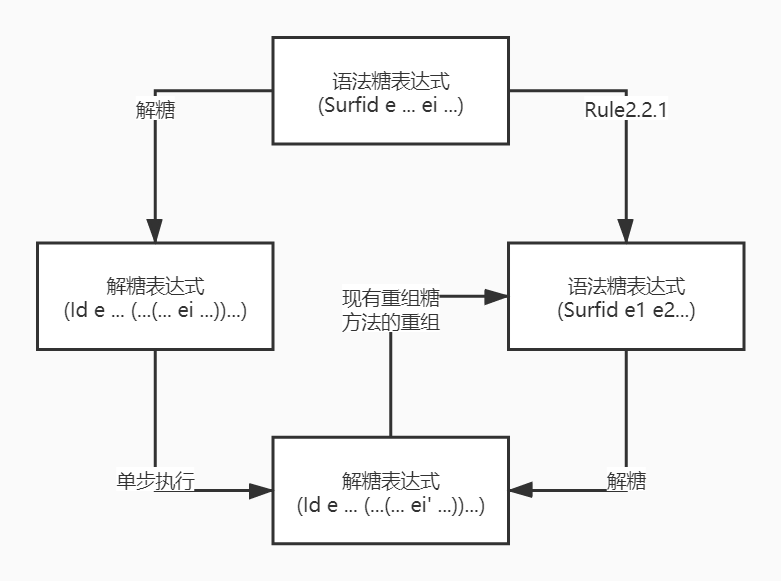
\includegraphics[width=12cm]{images/chapter3/flowgraph.jpg}
			\caption{Rule2.2.1仿真性图示}
			\label{fig:emulation}
		\end{figure}
		
		\item 如果DesugarExp'是$Surfexp$或$OtherSurfexp$,则此处将递归调用f,由于表达式深度有限,如果下层的表达式满足仿真性,则此处也满足仿真性.
	\end{itemize}

证毕。

\end{proof}






%如果被规约的子表达式是$Coreexp$或$Commonexp$,则和CoreLang上的表现一致;如果是$Surfexp$或$OtherSurfexp$,则相当于一个解糖操作,解糖是不影响仿真性的;而如果是




\subsection{抽象性}
抽象性:求值序列中只存在SurfLang中存在的术语,没有引入CoreLang中的术语。

抽象性的正确性是显然的,因为我们在每次输出都判断了输出的$Exp$是否是$Surfexp$或$Commonexp$。(在lightweight-resugaring算法中)

\subsection{覆盖性}
覆盖性:在求值序列中没有跳过一些中间过程。

\newtheorem{lemma}{引理}[section]

\begin{lemma}
	如果在重组糖序列中语法糖没有在不必须破坏的时候被破坏,那么就没有跳过中间过程。
\end{lemma}

\begin{proof}[引理证明]
	假设没有语法糖提前破坏的情况下,存在CoreLang序列中的某一项
	
	$Exp$=$(Headid\;Subexp_{1}\;Subexp_{\ldots} \ldots)$可被重组为
	
	$ResugarExp'$=$(Surfid\;Subexp'_{1}\;Subexp'_{\ldots}\ldots)$,且没有在算法lightweight-resugaring中被表现。则说明
	\begin{itemize}
		\item 或是重组糖序列中存在
		
		$ResugarExp$=$(Surfid\;Subexp'_{1}\;\ldots\;Subexp_{i}\;Subexp'_{\ldots}\ldots)$
		
		使得$ResugarExp$解糖后得到的表达式单步规约得到$Exp$,且此时该单步规约将$ResugarExp$中子表达式$Subexp_{i}$对应部分规约。我们发现此时$ResugarExp$的语法糖结构并没有被破坏,因此如果不能展示$ResugarExp'$则是提前破坏了不必要破坏的语法糖,与假设前提矛盾。
		
		\item 或是重组糖序列中存在
		
		$ResugarExp$=$(Surfid'\;\ldots\;ResugarExp'\;\ldots)$
		
		使得$ResugarExp$解糖后得到的表达式单步规约得到$Exp$,且该$Exp$是从$ResugarExp$中的子表达式$ResugarExp'$解糖得到,说明此步单步规约不涉及$ResugarExp'$的规约。而如果不能展示$ResugarExp'$,则说明该语法糖在执行前面的序列被提前破坏了,也与假设矛盾。

	\end{itemize}

证毕。
\end{proof}

\begin{mythm}[覆盖性]
	我们的轻量级重组糖具有覆盖性。
\end{mythm}

\begin{proof}
	由引理可知,只需证明核心算法f得每一条都不会将语法糖在不必要破坏时被破坏。
	对f的每一条进行讨论。
	
	对Rule1.1和Rule1.3显然没有破坏不必须破坏的语法糖。
	
	对Rule1.2,由于CoreLang的表达式需要进一步规约必须对特定子表达式进行规约,因此要对相应的下层表达式作用f。同仿真性,由于表达式深度有限,下层表达式作用f满足覆盖性可递归证明上层表达式满足覆盖性。
	
	对Rule2.1,此时必须破坏语法糖,否则无法继续规约。
	
	对Rule2.2.1,与Rule1.2相同,递归的对下层表达式作用f,递归证明覆盖性。
	
	对Rule2.2.2,因为单步尝试后发现语法糖解糖后,解糖后结构继续被破坏,因此无法还原回语法糖,也是必须破坏的语法糖。
	
	因此求值序列没有破坏任何不必须破坏的语法糖,核心算法f满足覆盖性。
\end{proof}




\section{Evaluation}

Explain how your system is implemented and how the experiment is performed to evaluate your approach.
%!TEX root = ./main.tex
\section{Implementation and Case Studies}
\label{sec5}


\subsection{Implementation}

Our resugaring approach is implemented using PLT Redex\cite{SEwPR}, which is a semantic engineering tool based on reduction semantics\cite{reduction}. The framework of the implementation is as Figure \ref{fig:frame}.
In the language model, desugaring rules are written as reduction rules of \m{SurfExp}. And context rules of \m{SurfExp} have no restriction (every subexpression is reducible as a hole). Then for each resugaring step, we should choose the exact reduction which satisfies the reduction of mixed language's reduction rule  in Section \ref{mark:mixedreduction}.
\begin{figure}[t]
	\centering
	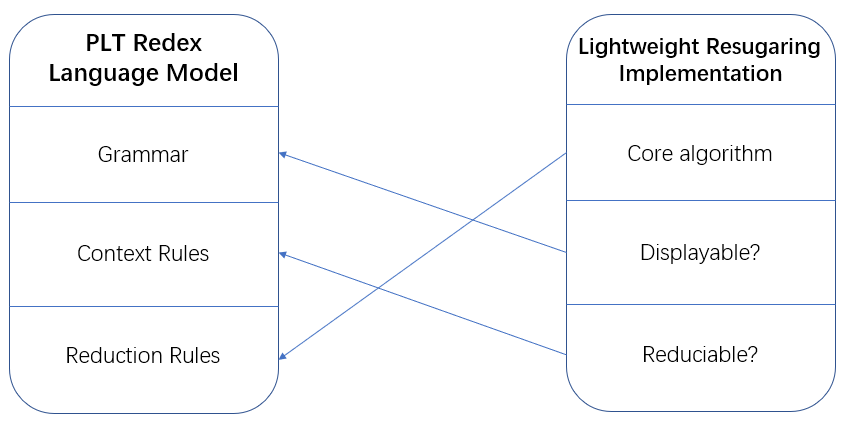
\includegraphics[width=5cm]{images/frame.png}
	\caption{Framework of Implementation}
	\label{fig:frame}
\end{figure}



\ignore{
\label{mark:blackbox}
And one may notice the traditional resugaring approach does not need the whole evaluation rules of core language, a black-box stepper is enough instead. Our approach can also work by  given a black-box stepper with a tricky extension, but a little more information is needed. Here we introduce the extension firstly.
We use $\redc{}{}$ to denote a reduction step of core language's expression in the black-box stepper, and $\rede{}{}$ to denote a step in the extension evaluator for the mixed language. We may use $\redm{}{}$ to denote the one-step reduction in our mixed language, defined in Section \ref{mark:mixedreduction}.
\infrule[CoreRed]
{ \forall~i.~e_i\in \m{CoreExp}\\
\redc{(\m{CoreHead}~e_1~\ldots~e_n)}{e'}}
{\rede{(\m{CoreHead}~e_1~\ldots~e_n)}{e'}}
\infrule[CoreExt1]
{ \forall~i.~tmp_i= (e_i \in \m{SurfExp}~?~\m{tmpe}~:~e_i),~where~\m{tmpe}~is~any~reduciable~\m{CoreExp}~term\\
\redc{(\m{CoreHead}~tmp_1~\ldots~tmp_i~\ldots~tmp_n)}{(\m{CoreHead}~tmp_1~\ldots~tmp_i'~\ldots~tmp_n)}}
{\rede{(\m{CoreHead}~e_1~\ldots~e_i~\ldots~e_n)}{(\m{CoreHead}~e_1~\ldots~e_i'~\ldots~e_n)}\\where~\redm{e_i}{e_i'}~if~e_i~\in~\m{SurfExp},~else~\rede{e_i}{e_i'}}
\infrule[CoreExt2]
{ \forall~i.~tmp_i= (e_i \in \m{SurfExp}~?~\m{tmpe}~:~e_i),~where~\m{tmpe}~is~any~reduciable~\m{CoreExp}~term\\
\redc{(\m{CoreHead}~tmp_1~\ldots~tmp_n)}{e'}~\note{// not reduced in subexpressions}}
{\rede{(\m{CoreHead}~e_1~\ldots~e_n)}{e'[e_1/tmp_1~\ldots~e_n/tmp_n]}}
Then we should replace the rules \m{CoreRed1} and \m{CoreRed2} by the following rule.
\infrule[ExtRed]
{\rede{(\m{CoreHead}~e_1~\ldots~e_n)}{e'}}
{\redm{(\m{CoreHead}~e_1~\ldots~e_n)}{e'}}

Putting them in simple words. For expression \Code{(CoreHead $e_1$ $\ldots$ $e_n$)} whose subexpressions contain \m{SurfExp}, replacing all \m{SurfExp} subexpressions not in core language with any reducible core language's term \m{tmpe}. Then getting a result after inputting the new expression $e'$ to the original black-box stepper. If reduction appears at a subexpression at $e_i$ or what the $e_i$ replaced by, then the stepper with the extension should return \Code{(CoreHead $e_1$ $\ldots$ $e_i'$ $\ldots$ $e_n$)}, where $e_i'$ is $e_i$ after the mixed language's one-step reduction ($\redm{}{}$) or after core language's reduction with extension ($\rede{}{}$) (rule \m{CoreExt1}, an example in Figure \ref{fig:e1}). Otherwise, the stepper should return \Code{$e'$}, with all the replaced subexpressions replacing back (rule \m{CoreExt2}, an example in Figure \ref{fig:e2}). The extension will not violate the properties of original core language's evaluator. It is obvious that the evaluator with the extension will reduce at the subexpression as it needs in core language, if the reduction appears in a subexpression. One may notice that the stepper with extension behaves the same as mixing the evaluation rules of core language and desugaring rules of surface language. The extension is just to make it works when the evaluator of core language is a black-box stepper, by getting context rules using the \m{tmpe}. That's why the extension is tricky.
\reduce{can be simplified}

\begin{center}
\begin{figure}[thb]
\centering
\Code{(if (and e1 e2) true false)}\\ $\Downarrow_{replace}$\\ \Code{(if tmpe1 true false)}\\ $\Downarrow_{blackbox}$\\ \Code{(if tmpe1' true false)}\\ $\Downarrow_{desugar}$\\ \Code{(if (if e1 e2 false) true false)}
\caption{\m{CoreExt1}'s Example}
\label{fig:e1}
\end{figure}

\begin{figure}[thb]
\centering
\Code{(if (if true ture false) (and ...) (or ...))}\\ $\Downarrow_{replace}$ \\\Code{ (if (if true ture false) tmpe2 tmpe3)}\\ $\Downarrow_{blackbox}$\\  \Code{(if true tmpe2 tmpe3)}\\ $\Downarrow_{replaceback}$\\ \Code{(if true (and ...) (or ...))}
\caption{\m{CoreExt2}'s Example}
\label{fig:e2}
\end{figure}


\end{center}

But something goes wrong when substitution takes place during \m{CoreExt2}. Just as the example we will talk about later in Section \ref{mark:hygienic}, for a expression like \Code{(let x 2 (Sugar x 1))}, it should reduce to \Code{(Sugar 2 1)} by the \m{CoreRed2} rule, but got \Code{(Sugar x 1)} by the \m{CoreExt2} rule. So when using the extension of black-box stepper's rule (\m{ExtRed2}), we need some other information about in which subexpression a substitution will take place (the substitution can be got by a similar idea as the tricky extension). Then for these subexpressions, we need to do the same substitution before replacing back.
}
% \todo{black-box's extension was removed, maybe add in appendix}



\label{mark:optimize}
Note that in \m{SurfRed1} rule and \m{CoreExt1} rule, there is a recursive call on $\redm{}{}$. We can optimize the resugaring algorithm by recursively resugaring. For example, \Code{(Sugar1 (Sugar2  ...) ...)} as the input, and find the first subexpression should be reduced. We can first get the resugaring sequences of \Code{(Sugar2 ...)} as Figure \ref{fig:subsequence}, then the resugaring sequences is got as \ref{fig:optimized}. Thus, we will not need to try to expand the outermost sugar for each inner step (recursively resugaring for inner expression).

\begin{figure}[t]
\centering
\subcaptionbox{Subsequences of \m{Sugar2} \label{fig:subsequence}}[.45\linewidth]{
\begin{flushleft}
{\small
\begin{Codes}
\qquad (Sugar2 ...)\\
  \OneStep{ exp1}\\
\DeStep{\quad expi} \note{//0 or more steps}\\
\OneStep{ expn}
\end{Codes}
}
\end{flushleft}
}
\subcaptionbox{Optimized Resugaring of \m{Sugar1} \label{fig:optimized}}[.45\linewidth]{
\begin{flushleft}
{\small
\begin{Codes}
\qquad (Sugar1 (Sugar2 ...) ...)\\
  \OneStep{ (Sugar1 exp1 ...)}\\
\DeStep{\quad(Sugar1 expi ...)} \note{//0 or more steps}\\
\OneStep{ (Sugar1 expn ...)}
\end{Codes}
}
\end{flushleft}
}
\caption{Recursive Optimization's Example}
\label{fig:optimize}
\end{figure}


As for the automatic derivation of evaluation rules, we implement a simple demo by writing some core language's IFAs (such as \m{if}, \m{let}) manually, because it is enough to do some case studies for the resugaring tasks.

\subsection{Case Studies}



We test some applications on the tool as case studies. Some examples we will discuss in this section are in Figure \ref{fig:resugaring}. Note that we set call-by-value lambda calculus as terms in \m{CommonExp}, because we need to output some intermediate sequences including lambda expressions in some examples. It's easy if we want to skip them. \todo{modify drule or simplify Codes}

\begin{figure}[t]
\centering
\subcaptionbox{Example of SKI\label{fig:SKI}}[.3\linewidth]{
\begin{flushleft}
{\scriptsize
\begin{Codes}
\qquad (S (K (S I)) K xx yy)\\
\OneStep{ (((K (S I)) xx (K xx)) yy)}\\
\OneStep{ (((S I) (K xx)) yy)}\\
\OneStep{ (I yy ((K xx) yy))}\\
\OneStep{ (yy ((K xx) yy))}\\
\OneStep{ (yy xx)}

\end{Codes}
}
\end{flushleft}
}
\subcaptionbox{Example of \m{Hygienicadd}\label{fig:hygienicadd}}[.32\linewidth]{
\begin{flushleft}
{\scriptsize
\begin{Codes}
\qquad    (let x 2 (Hygienicadd 1 x))\\
\OneStep{ (Hygienicadd 1 2)}\\
\OneStep{ (+ 1 2)}\\
\OneStep{ 3}\\

\end{Codes}

}
\end{flushleft}
}
\subcaptionbox{Example of \m{Let}\label{fig:Let}}[.36\linewidth]{
\begin{flushleft}
{\scriptsize
\begin{Codes}
\qquad    (Let x 1 (+ x (Let x 2 (+ x 1))))\\
\OneStep{ (Let x 1 (+ x (+ 2 1)))}\\
\OneStep{ (Let x 1 (+ x 3))}\\
\OneStep{ (+ 1 3)}\\
\OneStep{ 4}\\
\end{Codes}
}
\end{flushleft}
}

%newline
\subcaptionbox{Example of \m{Odd} and \m{Even}\label{fig:oddeven}}[.3\linewidth]{
\begin{flushleft}
{\scriptsize
\begin{Codes}
\qquad    (Odd 2)\\
\OneStep{ (Even (- 2 1))}\\
\OneStep{ (Even 1)}\\
\OneStep{ (Odd (- 1 1))}\\
\OneStep{ (Odd 0)}\\
\OneStep{ \#f}
\end{Codes}
}
\end{flushleft}
}
\subcaptionbox{Example of \m{Map}\label{fig:Map}}[.55\linewidth]{
\begin{flushleft}
{\scriptsize
\begin{Codes}
    \qquad(Map (lambda (x) (+ x 1)) (cons 1 (list 2)))\\
\OneStep{ (Map (lambda (x) (+ x 1)) (list 1 2))}\\
\OneStep{ (cons 2 (Map (lambda (x) (+ 1 x)) (list 2)))}\\
\OneStep{ (cons 2 (cons 3 (Map (lambda (x) (+ 1 x)) (list))))}\\
\OneStep{ (cons 2 (cons 3 (list)))}\\
\OneStep{ (cons 2 (list 3))}\\
\OneStep{ (list 2 3)}
\end{Codes}
}
\end{flushleft}
}
\subcaptionbox{Example of \m{Filter}\label{fig:Filter}}[.9\linewidth]{
\begin{flushleft}
{\scriptsize
\begin{Codes}
    \qquad(Filter (lambda (x) (and (> x 1) (< x 4))) (list 1 2 3 4))\\
\OneStep{ (Filter (lambda (x) (and (> x 1) (< x 4))) (list 2 3 4))}\\
\OneStep{ (cons 2 (Filter (lambda (x) (and (> x 1) (< x 4))) (list 3 4)))}\\
\OneStep{ (cons 2 (cons 3 (Filter (lambda (x) (and (> x 1) (< x 4))) (list 4))))}\\
\OneStep{ (cons 2 (cons 3 (Filter (lambda (x) (and (> x 1) (< x 4))) (list))))}\\
\OneStep{ (cons 2 (cons 3 (list)))}\\
\OneStep{ (cons 2 (list 3))}\\
\OneStep{ (list 2 3)}
\end{Codes}

}
\end{flushleft}
}
\caption{Resugaring Examples}
\label{fig:resugaring}
\end{figure}


\subsubsection{Simple sugar}
\label{mark:simple}

We construct some simple syntactic sugars and try it on our tool. Some sugar is inspired by the first work of resugaring\cite{resugaring}. The result shows that our approach can handle all sugar features of their first work.
Take an SKI combinator syntactic sugar as an example.
\[
\begin{array}{l}
\drule{\m{S}}{\Code{(lambdaN (x1 x2 x3) (x1 x2 (x1 x3)))}}\\
\drule{\m{K}}{\Code{(lambdaN (x1 x2) x1)}}\\
\drule{\m{I}}{\Code{(lambdaN (x) x)}}
\end{array}
\]




Although SKI combinator calculus is a reduced version of lambda calculus, we can construct combinators' sugar based on call-by-need lambda calculus in our core language. For sugar expression \Code{(S (K (S I)) K xx yy)}, we get the resugaring sequences as Figure \ref{fig:SKI}. During the test, we find 33 intermediate steps are needed after the totally desugaring of the input expression, but only 5 of them can be returned to the surface, so many attempts to reverse the desugaring would fail if using the traditional resugaring approach, in such a little expression. That's why lazy desugaring makes our approach efficient.




\ignore{
  For the traditional approach, the sugar expression should firstly desugar to
\begin{Codes}
((lambdaN (x1 x2 x3) (x1 x3 (x2 x3)))
  ((lambdaN (x1 x2) x1)
   ((lambdaN  (x1 x2 x3) (x1 x3 (x2 x3)))
    (lambdaN (x) x)))
  (lambdaN (x1 x2) x1)
  xx yy)
\end{Codes}
\reduce{can be removed}

Then in our core language, the execution of expanded expression will contain 33 reduction steps in our implementation. For each step, there will be many attempts to match and substitute the syntactic sugars to resugar the expression. It will omit more steps for a larger expression.
}

As for the derivation of syntactic sugar's evaluation rules, we have shown an example of \m{and} sugar and \m{or} sugar in overview. But what if the \m{or} sugar written as follows?
\[\drule{\Code{(or $e_1$ $e_2$)}}{\Code{(let x $e_1$ (if x x $e_2$))}}\]
Of course, we got the same evaluation rules as the example in overview.
\[
\begin{array}{c}
\infer {(\mbox{or}~e_1~e_2) \rightarrow (\mbox{or}~e_1'~e_2)} {e_1~ \rightarrow~e_1'}
\qquad
(\mbox{or}~\#t~e2) \rightarrow \#t
\quad
(\mbox{or}~\#f~e2) \rightarrow e_2 \\
\end{array}
\]

Then for expressions headed with \m{or}, we won't need the one-step try to figure out whether desugaring or processing on a subexpression, which makes our approach more concise. Overall, the unidirectional resugaring algorithm makes our approach efficient, because no attempts for resugaring the expression are needed.
\subsubsection{Hygienic sugar}
\label{mark:hygienic}


The second work\cite{hygienic} of traditional resugaring approach mainly processes hygienic sugar compared to first work. It uses a DAG to represent the expression. However, hygiene is not hard to be handled by our lazy desugaring strategy. Our algorithm can easily process hygienic sugar without a special data structure.
A typical hygienic problem is as the following example.
\[
\drule{\Code{(Hygienicadd $e_1$ $e_2$)}}{\Code{(let x $e_1$ (+ x $e_2$))}}
\]
% \begin{Codes}
% 	(Hygienicadd e1 e2) \DeStep{ (let ((x e1)) (+ x e2))}
% \end{Codes}
For traditional resugaring approach, if we want to get sequences of \Code{(let x 2 (Hygienicadd 1 x))}, it will firstly desugar to \Code{(let x 2 (let x 1 (+ x x)))}, which is awful because the two $x$ in \Code{(+ x x)} should be bind to different value. So the traditional hygienic resugaring approach uses abstract syntax DAG to distinct different \m{x} in the desugared expression. But for our approach based on lazy desugaring, the \m{hygienicadd} sugar does not have to desugar until necessary, thus, getting resugaring sequences as Figure \ref{fig:hygienicadd} based on a rewriting system which renaming the variables during the rewriting. \todo{@zc: different values?; what's  meaning of the sentence after "thus"}


The lazy desugaring is also convenient for hygienic resugaring for non-hygienic rewriting. For example, \Code{(let x 1 (+ x (let x 2 (+ x 1))))} may be reduced to \Code{(+ 1 (let 1 2 (+ 1 1)))} by a simple core language whose \Code{let} expression does not handle cases like that. But by writing a simple sugar Let,
\[\drule{\Code{(Let~$e_1$~$e_2$~$e_3$)}}{\Code{(let~($e_1$~$e_2$)~$e_3$)}}\]
and making some simple modifies in the reduction of mixed language, we will get the resugaring sequences as Figure \ref{fig:Let} in our tool. todo{@zc: let (e e) e -> let e e e; support Let now?}


In practical application, we think hygiene can be easily processed by rewriting systems, so we just use a rewriting system which can rename variable automatically.

And for the derivation method, there is no rewriting system at all, but the hygiene is handled more concisely. we build a hygienic sugar \m{Hygienicor} based on the \m{or} sugar.
\[
\begin{array}{l}
\drule{\Code{(Or $e_1$ $e_2$)}}{\Code{(let x $e_1$ (if x x $e_2$))}}\\
\drule{\Code{(Hygienicor $e_1$ $e_2$)}}{\Code{(let x $e_1$ (or $e_2$ x))}}
\end{array}
\]
Though no need to write the sugar like that, something wrong may happen without hygienic rewriting system (\Code{(if x x x)} appears). But with the step in normalization of IFA introduced in \ref{mark:hygieneinderive}, we can easily get the following rules, which will behave as it should be in resugaring. \todo{@zc: Because we have replaced x with expression when constructing normal IFA of or, the binding of x will not cause conflicts.}
\[
\begin{array}{c}
\infer {(\mbox{Hygienicor}~e_1~e_2) \rightarrow (\mbox{Hygienicor}~e_1'~e_2)} {e_1~ \rightarrow~e_1'}
\qquad
\infer {(\mbox{Hygienicor}~v_1~e_2) \rightarrow (\mbox{Hygienicor}~v_1~e_2')} {e_2~ \rightarrow~e_2'}
\end{array}\]
\[
\begin{array}{c}
(\mbox{Hygienicor}~v_1~\#t) \rightarrow \#t
\quad
(\mbox{Hygienicor}~v_1~\#f) \rightarrow v_1
\end{array}
\]

Overall, our result shows lazy desugaring is really a good way to handle hygienic sugar in any systems.

\subsubsection{Recursive sugar}
\label{sec:recursiveSugar}

Recursive sugar is a kind of syntactic sugars where call itself or each other during the expanding. For example,
\[
\begin{array}{l}
\drule{(\m{Odd}~$e$)~}{\Code{(if (> $e$ 0) (Even (- $e$ 1)) \false)}}\\
\drule{(\m{Even}~$e$)}{\Code{(if (> $e$ 0) (Odd (- $e$ 1)) \true)}}
\end{array}
\]
are common recursive sugars. The traditional resugaring approach can't process syntactic sugar written like this (non-pattern-based) easily, because boundary conditions are in the sugar itself.

Take \Code{(Odd 2)} as an example. The previous work will firstly desugar the expression using the rewriting system. Then the rewriting system will never terminate as following shows.
\begin{scriptsize}
\begin{Codes}
   (Odd 2)
\DeStep{ (if (> 2 0) (Even (- 2 1) \#f))}
\DeStep{ (if (> (- 2 1) 0) (Odd (- (- 2 1) 1) \#t))}
\DeStep{ (if (> (- (- 2 1) 1) 0) (Even (- (- (- 2 1) 1) 1) \#f))}
\DeStep{ ...}
\end{Codes}
\end{scriptsize}



Then the advantage of our approach is embodied. Our lightweight approach doesn't require a whole expanding of sugar expression, which gives the framework chances to judge boundary conditions in sugars themselves, and showing more intermediate sequences. We get the resugaring sequences as Figure \ref{fig:oddeven} of the former example using our tool.



We also construct some higher-order syntactic sugars and test them. The higher-order feature is important for constructing practical syntactic sugars. And many higher-order sugars should be constructed by recursive definition. The first sugar is \m{Filter}, implemented by pattern matching term rewriting.
\[\begin{array}{l}
\drule{\Code{(Filter $e$ (list $v_1$ $v_2$ ...))}}{}\\
\qquad\Code{(if ($e$ $v_1$) (cons $v_1$ (Filter $e$ (list $v_2$ ...)))\ (Filter $e$ (list $v_2$ ...)))}\\
\drule{\Code{(Filter $e$ (list))}}{\Code{(list)}}
\end{array}\]
and getting resugaring sequences as Figure \ref{fig:Filter}.
Here, although the sugar can be processed by traditional resugaring approach, it will be redundant. The reason is that, a Filter for a list of length $n$ will match to find possible resugaring $n*(n-1)/2$ times. Thus, lazy desugaring is really important to reduce the resugaring complexity of recursive sugar.

Moreover, just like the \emph{Odd and Even} sugar above, there are some simple rewriting systems which do not allow pattern-based rewriting. Or there are some sugars that need to be expressed by the terms in core language as rewriting conditions. Take the example of another higher-order sugar \m{Map} as an example, and get resugaring sequences as Figure \ref{fig:Map}.
\[
\begin{array}{l}
\drule{\Code{(Map $e_1$ $e_2$)}}{}\\
\Code{(let x $e_2$ (if (empty? x) (list) (cons ($e_1$ (first x)) (Map $e_1$ (rest x)))))}
\end{array}
\]



Note that the \m{let} term is to limit the subexpression only appears once in RHS. In this example, we can find that the list \Code{(cons 1 (list 2))}, though equal to \Code{(list 1 2)}, is represented by core language's term. So it will be difficult to handle such inline boundary conditions for traditional rewriting systems. But our approach is easy to handle cases like this. So our resugaring approach by lazy desugaring is powerful.

\todo{@zc: whether it is necessary to discuss ifa cannot do this}

%!TEX root = ./main.tex
\section{Conclusion}
\label{sec7}

%Summarize the paper, explaining what you have shown, what results you have achieved, and what future work is.

In this paper, we propose a novel resugaring approach using lazy desugaring. We design the approach based on a  core language, with a simple desugaring system. Our algorithm then can output the evaluation sequence in the surface syntax, given some syntactic sugars together with an input program. In our approach, the most important insight is delaying the expansion of syntactic sugars by calculating context rules (Section \ref{sec:language} and \ref{sec:algo}), which decide whether the mixed language should reduce the sub-expression by core's reduction rules or expand the sugar. We show that the system can handle a variety of syntactic sugars and can achieve better efficiency (Section \ref{mark:resugaringexample} and \ref{sec:implementation}). Moreover, the approach is flexible to make some extensions (Section \ref{sec:ext}).

We find the extensions may work if the core language and the syntactic sugar have some properties such like compositional, clear semantics, and unique computational order. So one possible future work of this is to extend the core language and the desugaring system with other components of language design like type system, analyzer, and optimizer. Also, we find it is possible to derive stand-alone evaluation rules for the surface language by means similar to how we calculate context rules, making it more convenient to develop domain-specific languages. This functionality can be added to future systems.

%\chapter{章节名称}
\section{一级段落名称}
\subsection{二级段落名称}
\subsubsection{三级段落名称}
引用如\upcite{PhysRev.47.777},引用表如表\ref{tab:input_output_r},引用图如图\ref{fig:sample}.

\begin{table}[h]
	\small %内容,(五号,宋体/Time new roman)
	\centering
	\caption{不同频率下的输入和输出阻抗}
	\label{tab:input_output_r}
	\begin{tabular}{cccc} %表格使用三线表
		\toprule %不确定说明中三条线的粗细,待改
		频率(Hz) & 1 & 10k & 1M \\
		\midrule
		输入电阻($\Omega/^\circ$) & 339.719k/-87.84 & 5.6707k/-9.827 & 351.188/-72.377\\
		输出电阻($\Omega/^\circ$) & 338.638k/-89.663 & 1.9866k/-1.1228 & 1.9189k/-14.801 \\
		\bottomrule
	\end{tabular}
\end{table}

\begin{figure}[h]
	\centering
	\includegraphics[width=12cm]{sample.jpg}
	\caption{示例图片}
	\label{fig:sample}
\end{figure}
\clearpage



\chapter*{参考文献}
\noindent
\begin{enumerate}[{[1]}]
\small
	\item 期刊
	\item 网络文档
\end{enumerate}

1.	期刊  作者. 论文名. 刊名, 出版年份, 卷号(期号): 起始-截止页

2.	专著  作者. 书名. 版本(第一版不写). 出版城市: 出版社, 出版年份: 起始-截止页

3.	论文集  论文作者. 论文题目//编者. 论文集名: 其他题名信息. 出版城市(或者会议城市): 出版者, 出版年: 引文起始-截止页码

4.	学位论文  作者. 学位论文题名. 城市: 论文保存单位, 年份

5.	网络文献  作者. 题名[文献类型标志/文献载体标志]. 出版地: 出版者, 出版年(更新日期)[引用日期]. 获取和访问路径

*注意: 作者姓前名后, 超过3名作者列前3名, 后加“, 等”; 英文姓名, 姓前名后, 姓首字母大写, 名缩写; 文献的项目要完整, 各项的顺序和标点要和格式要求一致; 未公开发表的论文、报告不列入正式文献, 如有必要可在正文当页下加注。英文文献格式同上。参考文献在正文中按出现顺序用[1], [2]......在右上角标注, 放在“参考文献”中时, 用[1], [2], ...顺序标注。



\addcontentsline{toc}{chapter}{参考文献}
\fancypagestyle{plain}
{
	\fancyhf{}
	\fancyhead[RE,RO]{参考文献}
	\fancyhead[LE,LO]{北京大学本科生毕业论文}
	\fancyfoot[CO,CE]{~\thepage~}
	\renewcommand{\headrulewidth}{0.7pt}
	\renewcommand{\footrulewidth}{0pt}
}
\fancyhf{}
\fancyhead[RE,RO]{参考文献}
\fancyhead[LE,LO]{北京大学本科生毕业论文}
\fancyfoot[CO,CE]{~\thepage~}
\renewcommand{\headrulewidth}{0.7pt}
\renewcommand{\footrulewidth}{0pt}





\bibliographystyle{gbt7714-numerical}

\bibliography{ref}
这是参考“参考文献”,主要用来看引用的顺序,请手动些参考文献或自行写程序,最终编译请删除
\clearpage





\linespread{1}\selectfont
\normalsize
%小四号,中文宋体,英文Time new roman,1倍行距
\chapter*{本科期间的主要工作和成果}

\noindent 本科期间参加的主要科研项目

\noindent 本研基金
\begin{enumerate}
	\item 基金名称. 基金类型. 指导老师. 基金支持年限
\end{enumerate}

\noindent 各种科研项目
\begin{enumerate}
	\item 项目名称. 项目类型
\end{enumerate}

格式下

期刊:

全部作者. 论文名. 期刊名, 出版年份, 卷号(期号): 起始-截止页

会议论文:

全部作者. 论文名. 会议名, 会议举办地, 会议举办时间, 起始-截止页

专利

全部专利申请人. 专利名称. 专利申请号. 专利申请日期. 国别



\addcontentsline{toc}{chapter}{本科期间的主要工作和成果}
\fancypagestyle{plain}
{
	\fancyhf{}
	\fancyhead[RE,RO]{本科期间的主要工作和成果}
	\fancyhead[LE,LO]{北京大学本科生毕业论文}
	\fancyfoot[CO,CE]{~\thepage~}
	\renewcommand{\headrulewidth}{0.7pt}
	\renewcommand{\footrulewidth}{0pt}
}
\fancyhf{}
\fancyhead[RE,RO]{本科期间的主要工作和成果}
\fancyhead[LE,LO]{北京大学本科生毕业论文}
\fancyfoot[CO,CE]{~\thepage~}
\renewcommand{\headrulewidth}{0.7pt}
\renewcommand{\footrulewidth}{0pt}
\clearpage





\linespread{1.5}\selectfont
\normalsize
%正文,小四号,中文宋体,英文Time new roman,1.5倍行距
\chapter*{致谢}



\addcontentsline{toc}{chapter}{致谢}
\fancypagestyle{plain}
{
	\fancyhf{}
	\fancyhead[RE,RO]{致谢}
	\fancyhead[LE,LO]{北京大学本科生毕业论文}
	\fancyfoot[CO,CE]{~\thepage~}
	\renewcommand{\headrulewidth}{0.7pt}
	\renewcommand{\footrulewidth}{0pt}
}
\fancyhf{}
\fancyhead[RE,RO]{致谢}
\fancyhead[LE,LO]{北京大学本科生毕业论文}
\fancyfoot[CO,CE]{~\thepage~}
\renewcommand{\headrulewidth}{0.7pt}
\renewcommand{\footrulewidth}{0pt}





\end{document}
